\documentclass{beamer}
\mode<presentation>
\usepackage{tikz}
\usepackage{graphicx}
\usetikzlibrary{positioning}
\usefonttheme{professionalfonts}
\usetheme{Orr}
\usepackage[orientation=portrait,width=1m,height=1.2m,scale=1.4]{beamerposter}
\title{Phylogenies derived from somatic mutations agree with physical topologies in \textit{Eucalyptus}}
\titlegraphic{
	
\includegraphics[width=.95\linewidth]{figures/sols_logo.pdf}
	}
\date{4/8/16}
\author{Adam J Orr \inst{1,2} \and Robert Lanfear \inst{3,4} \and Reed Cartwright \inst{1,2}}
\institute{\inst{1} School of Life Sciences, Arizona State University \\
		   \inst{2} Biodesign Institute, Arizona State University \\
		   \inst{3} Department of Biological Sciences, Macquarie University \\
		   \inst{4} College of Medicine, Biology and Environment, Australian National University}
\email{ajorr1@asu.edu}
\website{cartwrig.ht/lab/}

\begin{document}

\begin{frame}{}
\begin{columns}

%%%% Left side %%%%

\column{.5\linewidth}

%%%%%%%%%%%%%%%%%%%

\begin{block}{\large Abstract}
\textit{Eucalyptus melliodora}, a tree native to eastern Australia, has strong timber and a high nectar load, making it economically important and a vital source of food for nectar-consuming species. In 1993, an individual of the species was discovered that harbors a somatic change conferring herbivore resistance to a section of branches on the tree via differential terpenoid production. Though transcriptomic analysis was inconclusive in determining the genetic source of this variation, we attempt to do so using ultra-deep whole-genome sequencing of 8 samples in triplicate. We call variants using a reference-free De-Bruijn variant caller \textit{DiscoSNP++} and by the GATK best practices using a reference from a closely-related species. We find that the phylogeny of the variants identified by both methods reflects the branching pattern of the tree, though the phylogeny is affected by short interior nodes. While we have yet to validate the source of the herbivore resistance, this data presents an opportunity for further study of how somatic mutations are produced and spread in plants and how to properly resolve short interior nodes.
\end{block}


\begin{block}{Introduction}

\begin{itemize}
\item Somatic mutations are rare but sequencing errors are common, making somatic mutations difficult to detect.
\item Little is known about the spread of somatic mutations, despite the key role they play in cancer development.
\item If the pattern of mutations in the phylogeny matches the branching pattern of the plant, then plants can be used to easily validate somatic mutations.
\end{itemize}

\end{block}





\begin{block}{Methods: Variant Detection}

\includegraphics[width=.97\linewidth]{figures/labeled_tree.jpg}

\vskip 2ex

\begin{itemize}
\item Samples 1-8 were collected in triplicate
\item Each replicate was Illumina sequenced
\item Each sequence was aligned to genome of \textit{Eucalyptus grandis} using bwa mem.
\item Variants were called using GATK's UnifiedGenotyper or DiscoSNP++, a reference-free variant caller
\item Nonvariable sites and gaps were removed
\item Variants were removed if the genotypes of all replicates of a sample were not identical
% \item Use RAxML to construct a tree.
\item A maximum likelihood tree was constructed with RAxML
\end{itemize}

\vskip 4ex

\begin{center}
	\begin{tikzpicture}[sqnode/.style={rectangle,draw=black!60,fill=black!5,very thick,minimum size=1cm}]
		\node[sqnode] (sequencing) {Sequence};
		\node[sqnode] (alignment) [below left = of sequencing] {Alignment};
		\node[sqnode] (gatk) [below = of alignment] {Get Variants (GATK)};
		\node[sqnode] (discosnp) [below right = of sequencing] {Get Variants (DiscoSNP++)};
		\node[sqnode] (filter) [below right = of gatk] {Filter};
		\node[sqnode] (tree) [below = of filter] {Tree Construction};
		\draw[ultra thick,->] (sequencing) -- (alignment);
		\draw[ultra thick,->] (sequencing) -- (discosnp);
		\draw[ultra thick,->] (alignment) -- (gatk);
		\draw[ultra thick,->] (gatk) -- (filter);
		\draw[ultra thick,->] (discosnp) -- (filter);
		\draw[ultra thick,->] (filter) -- (tree);
	\end{tikzpicture}
\end{center}


\end{block}




%%% Right Side %%%%

\column{.5\linewidth}

%%%%%%%%%%%%%%%%%%%

% \begin{block}{Methods: Reference Improvement}

% \begin{center}
% 	\begin{tikzpicture}[cnode/.style={rectangle,draw=black!60,fill=black!5,very thick}, node distance = .5 cm]
% 		\node[cnode] (reads){Reads};
% 		\node[cnode] (eg)[below = of reads]{E. grandis};
% 		\node[cnode] (em1)[right = of eg]{E. melliodora 1};
% 		\node[cnode] (em2)[right = of em1]{E. melliodora 2};
% 		\node[cnode] (etc)[right = of em2] {...};
% 		\draw[very thick,->] (reads) to [out=180,in=180] (eg);
% 		\draw[very thick,->] (reads) to (em1);
% 		\draw[very thick,->] (eg) -- (em1);
% 		\draw[very thick,->] (em1) -- (em2);
% 		\draw[very thick,->] (em2) -- (etc);
% 	\end{tikzpicture}
% \end{center}

% \end{block}



\begin{block}{Results: Variant Detection}

\begin{itemize}
\item The toplogy of the tree built from variants called by reference-free method DiscoSNP++ closely resembles the branching pattern of the plant.
\vskip 1ex
\item Its performance matches that of GATK used with a reference from the closely-related species \textit{Eucalyptus grandis}.
\vskip 1ex
\item A short internode causes incorrect placement of branches 6, 7, and 8 for both methods.
\end{itemize}

\vskip 3ex

\begin{columns}
	\column{.3\linewidth}
	\begin{block}{Tree Created with Variants From GATK}
	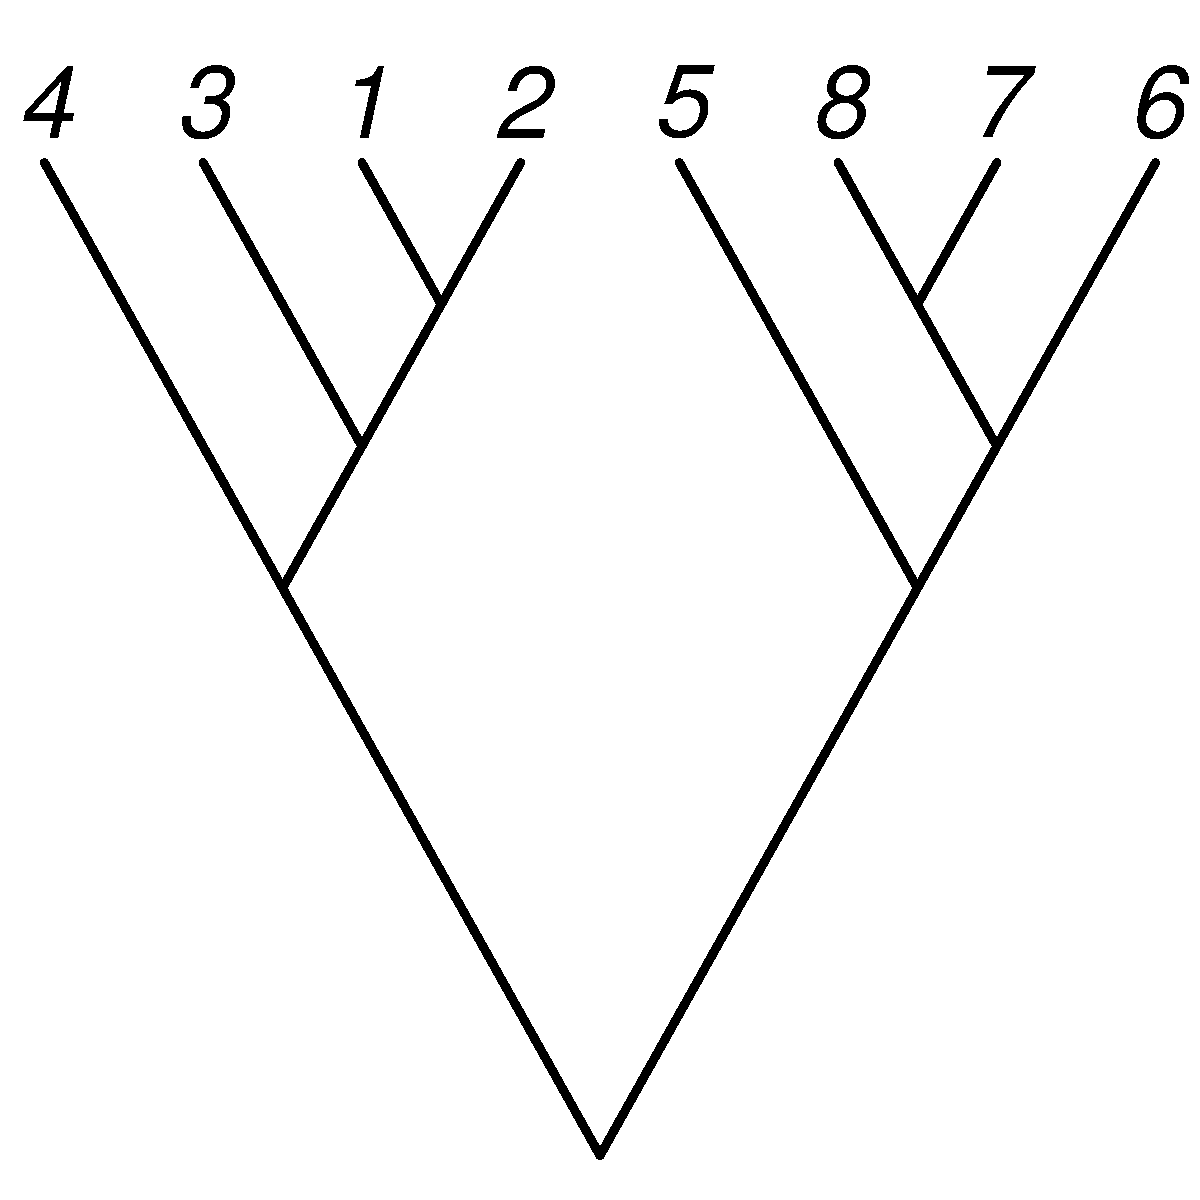
\includegraphics[width=.95\linewidth]{figures/gatk_tree.pdf}
	\end{block}
	\column{.3\linewidth}
	\begin{block}{Tree Created with Variants From DiscoSNP++}
	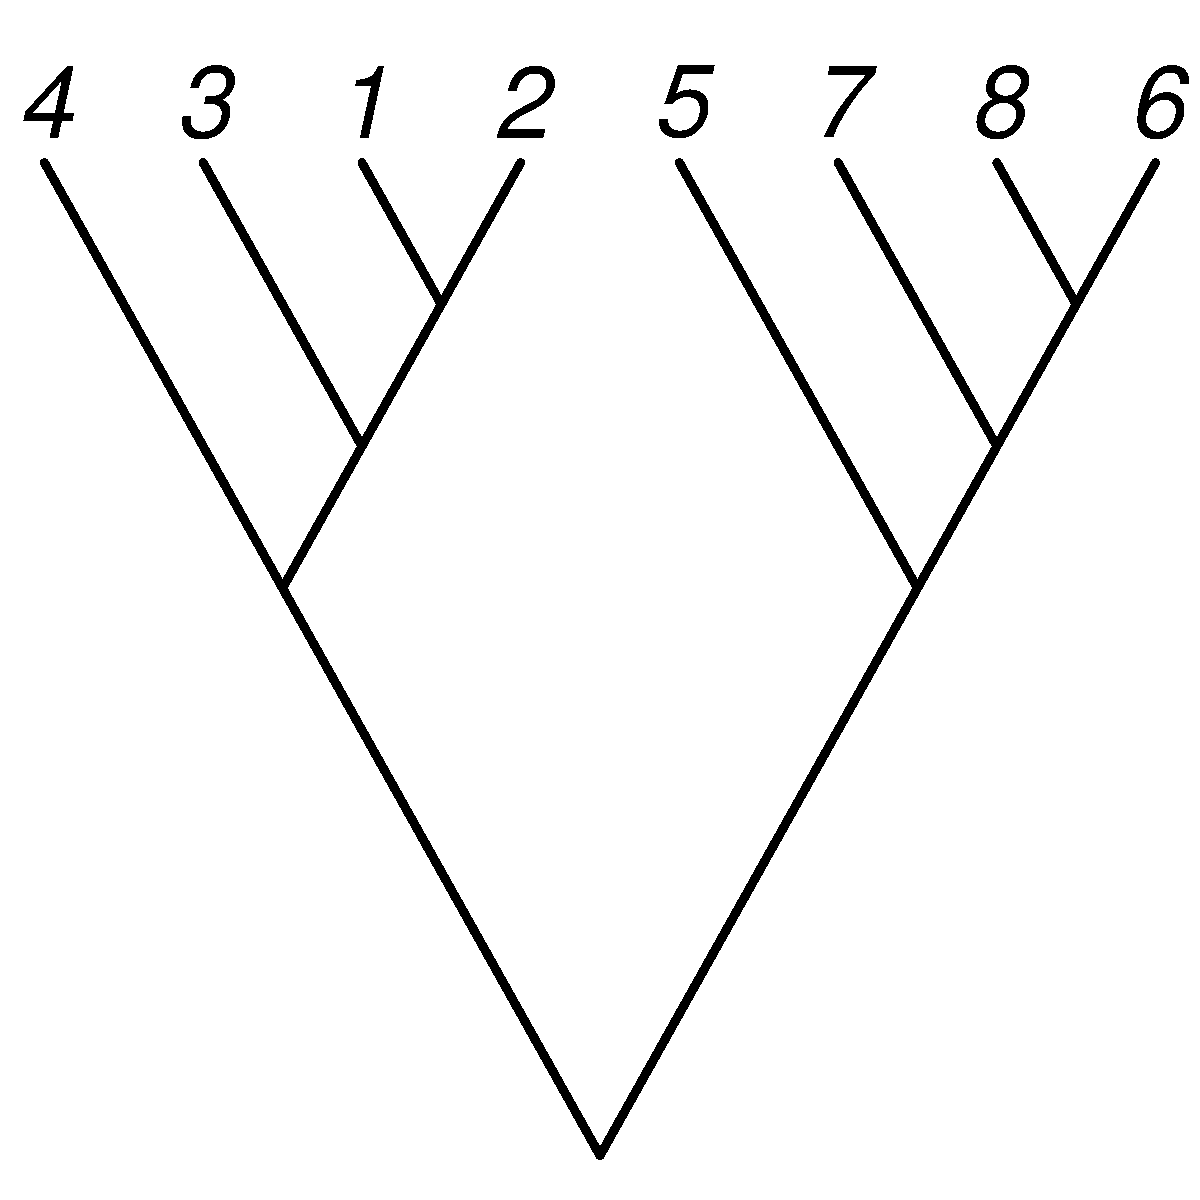
\includegraphics[width=.95\linewidth]{figures/disco_tree.pdf}
	\end{block}
	\column{.3\linewidth}
	\begin{block}{True Topology}
	\begin{center}
	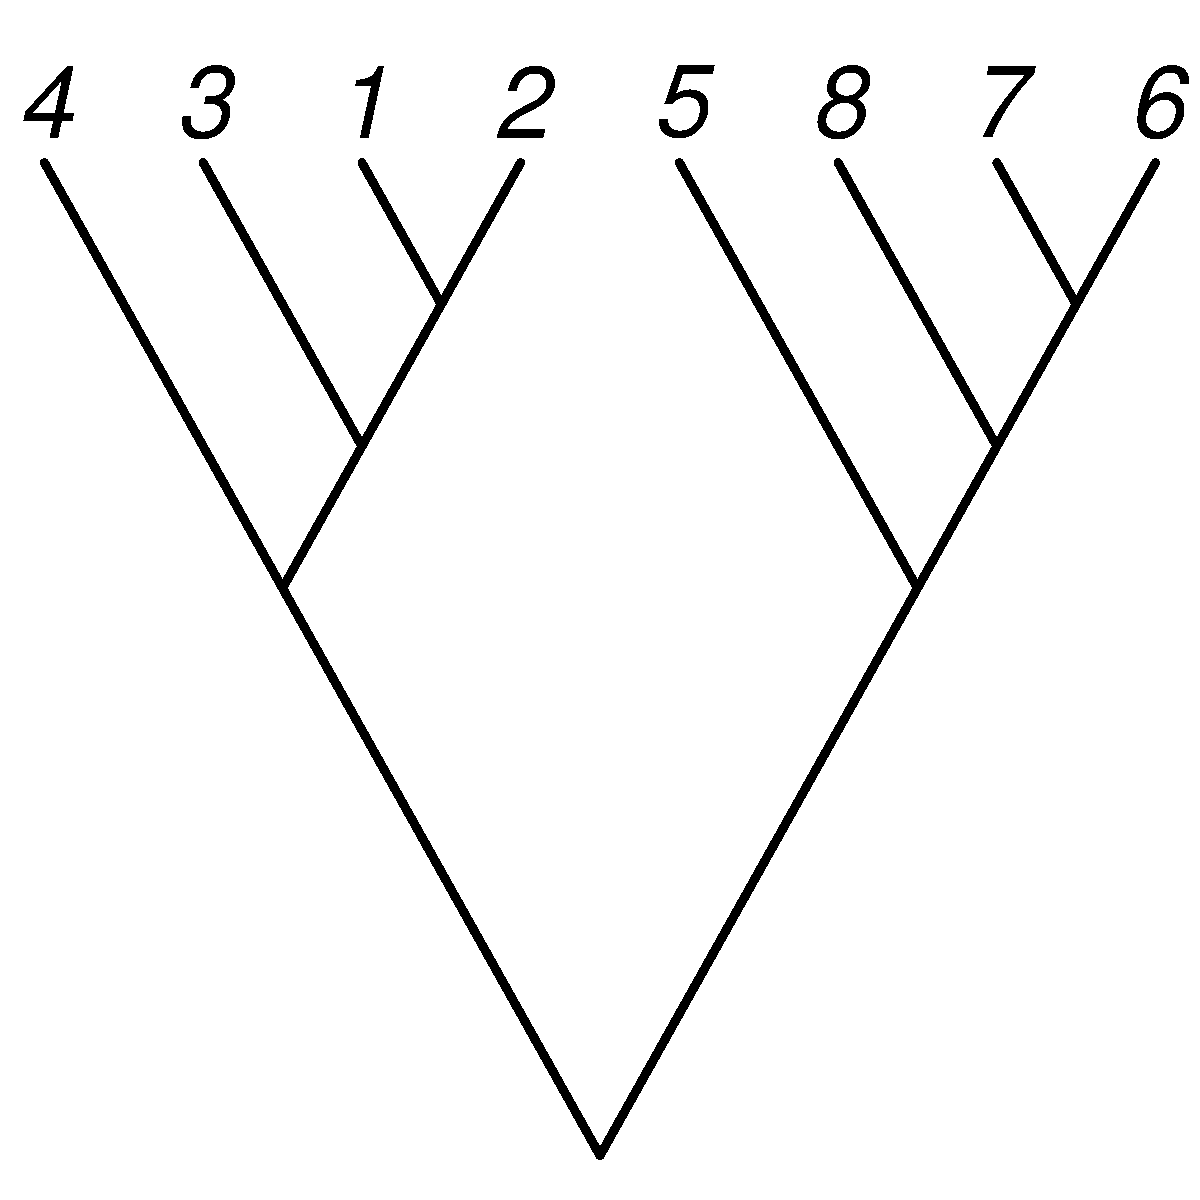
\includegraphics[width=.95\linewidth]{figures/true_tree.pdf}
	\end{center}
	\end{block}
\end{columns}

\end{block}


\begin{block}{Next steps: Reference Improvement}

To improve resolution of short internodes, we attempt to modify the
\textit{E. grandis} genome to make it more suitable for \textit{E. melliodora} by:

\begin{itemize}
\item Aligning the reads to the \textit{E. grandis} genome
\item Creating a consensus sequence from this alignment
\item Aligning the reads to this consensus to create a draft \textit{E. melliodora} genome
\end{itemize}

\vskip 2ex

\begin{center}
	\begin{tikzpicture}[cnode/.style={rectangle,draw=black!60,fill=black!5,very thick}, node distance = .5 cm]
		\node[cnode] (reads){Reads};
		\node[cnode] (eg)[below = of reads]{E. grandis};
		\node[cnode] (em1)[right = of eg]{E. melliodora 1};
		\node[cnode] (em2)[right = of em1]{E. melliodora 2};
		\node[cnode] (etc)[right = of em2] {...};
		\draw[very thick,->] (reads.west) to [out=180,in=180] (eg.west);
		\draw[very thick,->] (reads.east) to [out=0,in=90] (em1.north);
		\draw[very thick,->] (eg) -- (em1);
		\draw[very thick,->] (em1) -- (em2);
		\draw[very thick,->] (em2) -- (etc);
	\end{tikzpicture}
\end{center}

\end{block}


\begin{block}{Results: Reference Improvement}

\begin{center}

\includegraphics[width=.95\linewidth]{figures/both_hist.pdf}

\end{center}

\vskip 2ex

Alignment to the consensus sequence produces an alignment with higher overall quality scores than alignment to the \textit{Eucalyptus grandis} reference.

\end{block}


\begin{block}{Conclusions}

\begin{itemize}
	\item Phylogenies of somatic mutations within a \textit{Eucalyptus} tree match the branching patterns of the tree using both a reference-based and a reference-free variant caller.
	\item Aligning reads to a close relative, obtaining a consensus sequence, then realigning to that consensus seems to improve alignment quality.
\end{itemize}

\end{block}


\begin{block}{Acknowledgements}

\begin{center}
This work is supported by grant NIH R01-HG007178.

\vskip 1ex

\begin{columns}
\column{.3\linewidth}

\includegraphics[width=\linewidth]{figures/lab_logo.pdf}
\column{.3\linewidth}

\includegraphics[width=\linewidth]{figures/biodesign_logo.pdf}
\column{.2\linewidth}

\includegraphics[width=\linewidth]{figures/nih-nhgri-official-logo.jpg}
\end{columns}

\end{center}

\end{block}

\end{columns}
\end{frame}

% \begin{frame}{Broad Implications}
% 	\begin{itemize}
% 	\item How do somatic mutations spread? How can we study this?
% 	\item Cancers and other somatic diseases.
% 	\item A tree as a system for studying somatic mutation.
% 	\item The tree has a built-in point of reference
% 	\end{itemize}

% 	% \begin{alertblock}{A phylogeny is a \textbf{hypothesis}!}
% 	% 	We use simulations because we can't know the truth

% 	% 	Knowing the truth will allow us to evaluate phylogenetic tools		
% 	% \end{alertblock}

% \end{frame}

% \begin{frame}
% \begin{center}
% What mutation is causing the herbivore resistance phenotype?
% \end{center}
% \end{frame}


% %%A slide about cancer. Can we extract all the populations out of a tumor? Can we use a sequencing strategy to identify human GT vs cancer GT?

% %%We believe it to be the case that flowers & reproductive cells are forming as the branch forms, not transported through a stem-cell store.

% \begin{frame}{Somatic mutations are hard to find}
% Mutations are very rare, but sequencing errors are very common.
% \begin{itemize}
% \item Errors accumulate during PCR prior to sequencing - then propagate
% \item Errors accumulate in amplification steps during sequencing
% \item Technical error from sequencer
% \end{itemize}

% \textbf{Sequencer error} alone is \textbf{$\sim10^{-2}$} while mutation rate after error-checking is \textbf{$\sim10^{-10}$}

% \end{frame}

% %TODO: Need a sideways tree, a dendogram, and a normal tree

% \begin{frame}{Mutation Pattern Approximately Matches Tree Structure}
% \begin{columns}
% \column{.5\linewidth}
% 	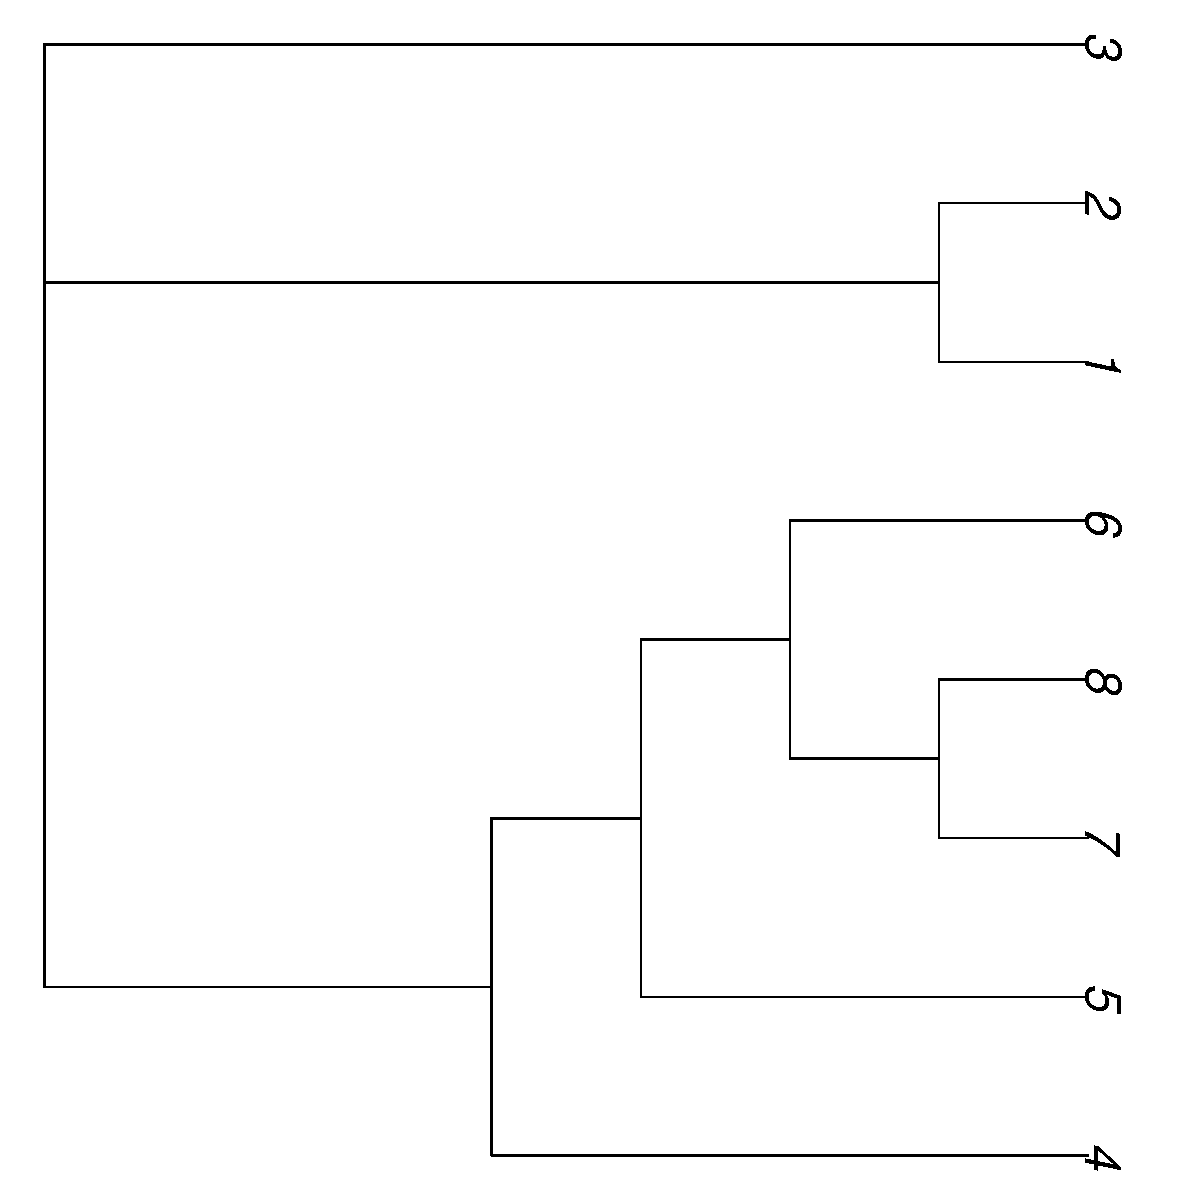
\includegraphics[width=\linewidth,angle=90]{../../../talks/eucalyptus/colloquium_2016/figures/gatk_tree_rotated.pdf}
% \column{.5\linewidth}
% 	\includegraphics[width=\linewidth]{../../../talks/eucalyptus/colloquium_2016/figures/labeled_tree.jpg}
% \end{columns}
% \end{frame}

% \begin{frame}{Most Reads Are Not Mapped to the \textit{E. grandis} Reference}
% \begin{center}
% 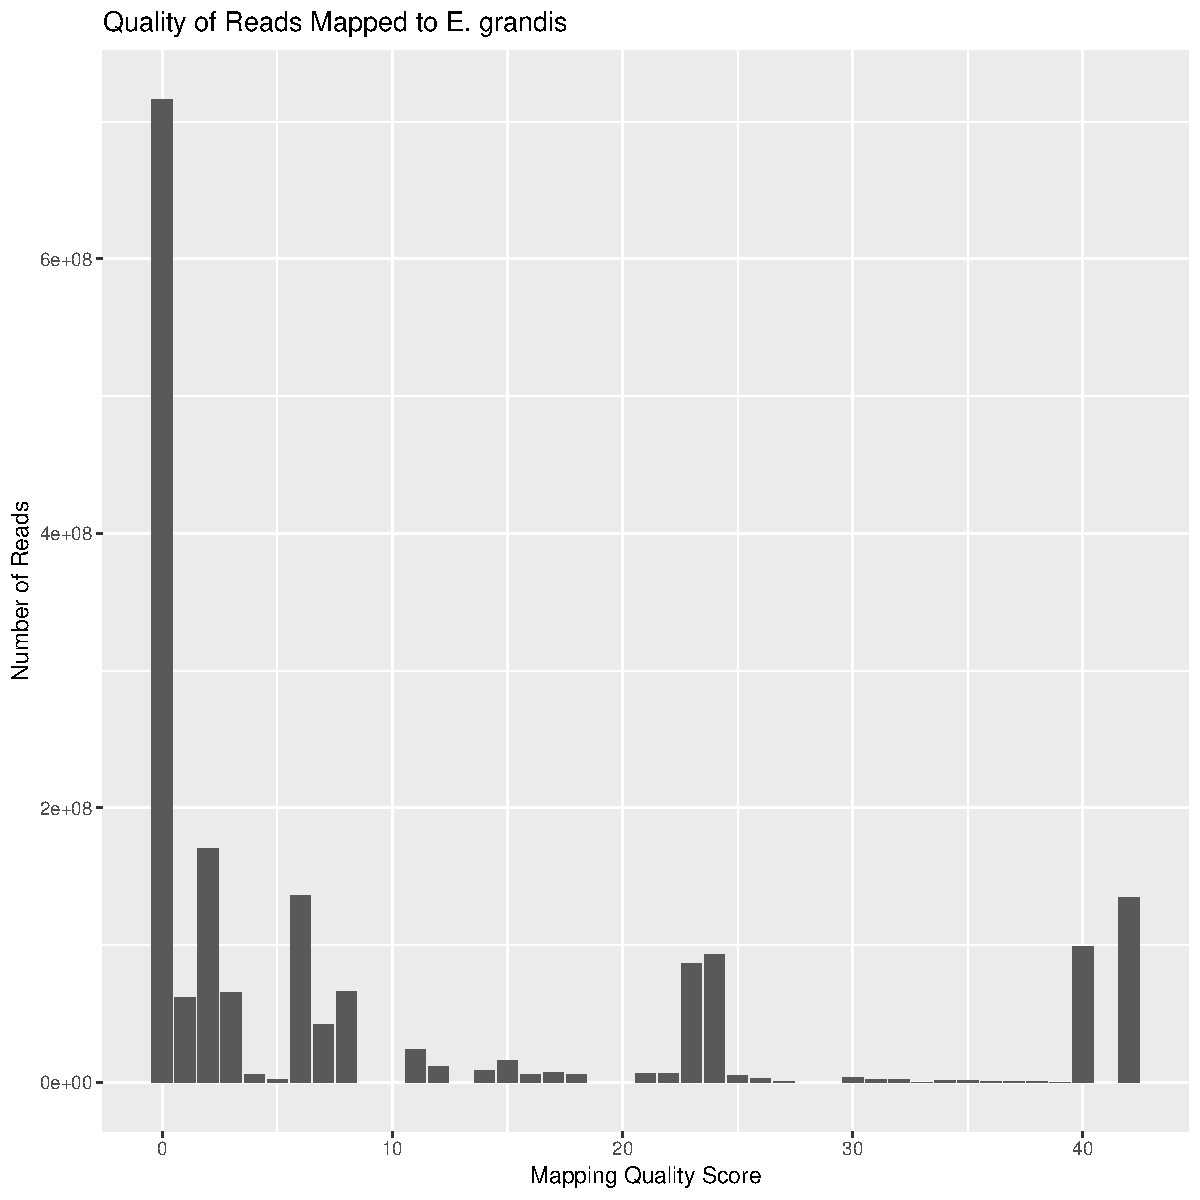
\includegraphics[height=.9\textheight]{../../../talks/eucalyptus/colloquium_2016/figures/bowtie1_hist.pdf}
% \end{center}
% \end{frame}

% \begin{frame}{A Reference-Free Method}
% \begin{columns}
% \column{.5\linewidth}
% \begin{center}
% \begin{tikzpicture}[sqnode/.style={rectangle, draw=black!60, fill=black!5,very thick,minimum size=1cm}]
% 	\node[sqnode] (sequencing) {Sequence};
% 	\node[sqnode] (alignment) [below = of sequencing] {Alignment};
% 	\node[sqnode] (varcall) [below = of alignment] {Get Variants (GATK)};
% 	\node[sqnode] (flt) [below = of varcall] {Filter};
% 	\draw[ultra thick,->] (sequencing.south) -- (alignment.north);
% 	\draw[ultra thick,->] (alignment.south) -- (varcall.north);
% 	\draw[ultra thick,->] (varcall.south) -- (flt.north);
% \end{tikzpicture}
% \end{center}
% \column{.5\linewidth}
% \begin{center}
% \begin{tikzpicture}[sqnode/.style={rectangle, draw=black!60, fill=black!5,very thick,minimum size=1cm}, gnode/.style={rectangle, draw = black!20, thick, minimum size=1cm}]
% 	\node[sqnode] (sequencing) {Sequence};
% 	\node[gnode] (alignment) [below = of sequencing] {Alignment};
% 	\node[sqnode] (varcall) [below = of alignment] {Get Variants (GATK)};
% 	\node[sqnode] (flt) [below = of varcall] {Filter};
% 	\draw[ultra thick,->] (sequencing.south) -- (varcall);
% 	\draw[ultra thick,->] (varcall.south) -- (flt.north);
% \end{tikzpicture}
% \end{center}
% \end{columns}
% \end{frame}


% \begin{frame}{The Reference-Free Method Performs Similarly}
% 	\begin{columns}
% 	\column{.5\linewidth}
% 		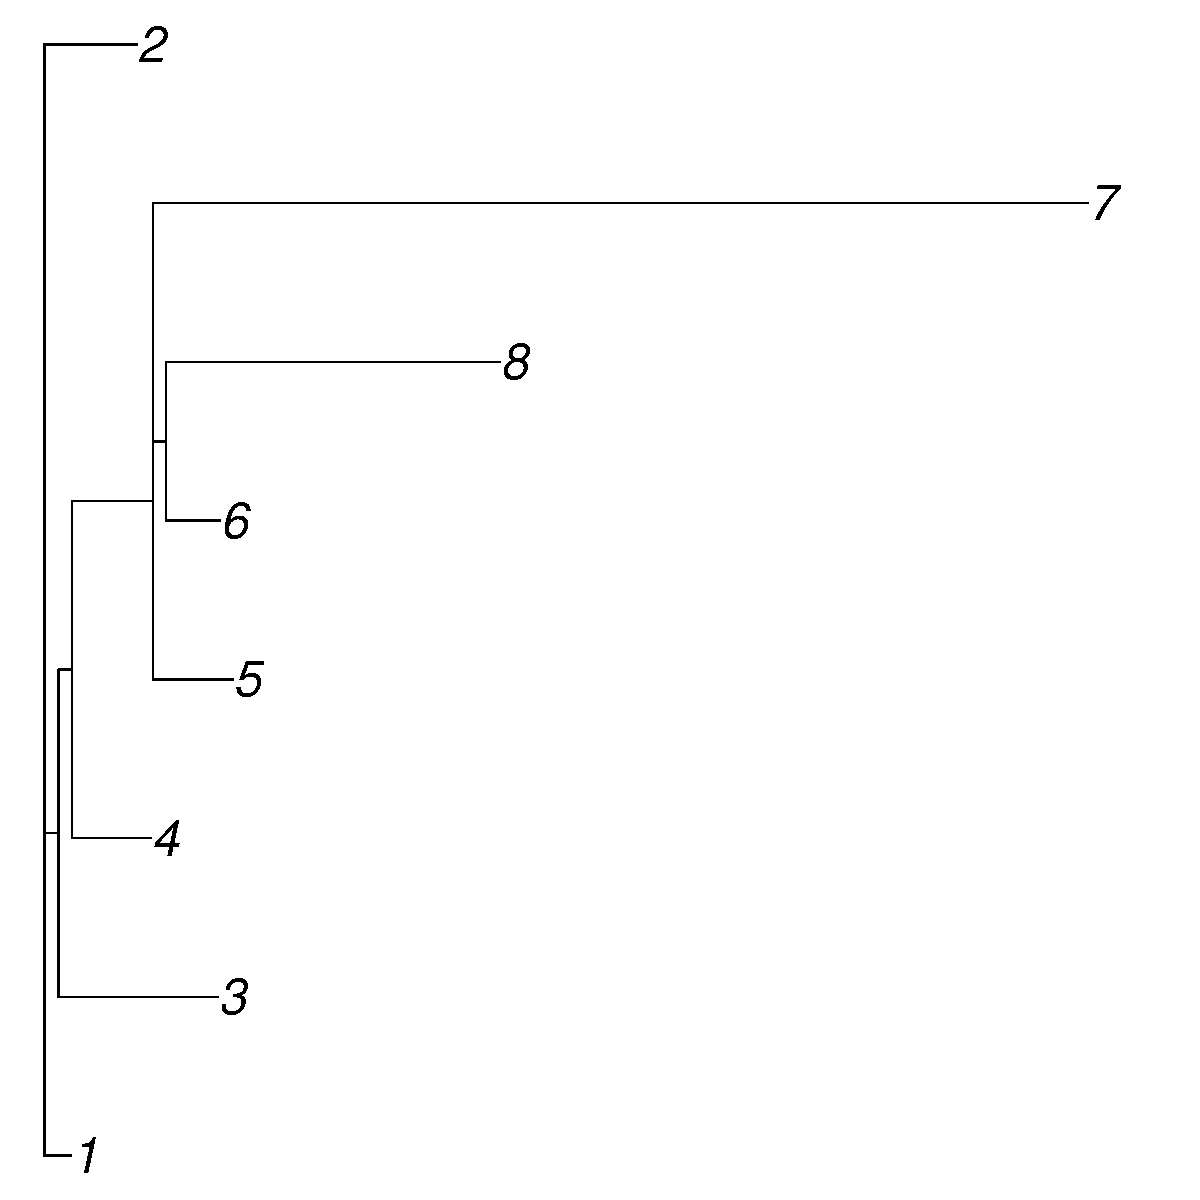
\includegraphics[width=\linewidth]{../../../talks/eucalyptus/colloquium_2016/figures/disco_tree2.pdf}
% 	\column{.5\linewidth}
% 		\includegraphics[width=\linewidth]{../../../talks/eucalyptus/colloquium_2016/figures/labeled_tree.jpg}
% 	\end{columns}
% \end{frame}

% % \begin{frame}{The Genome Analysis Toolkit}
% % 	\begin{itemize}
% % 	\item Used a traditional variant-calling pipeline: GATK best practices workflow
% % 	\item Reference genome of a close relative: \textit{Eucalyptus Grandis}
% % 	\end{itemize}
% % 	\begin{columns}
% % 	\column{.5\linewidth}
% % 		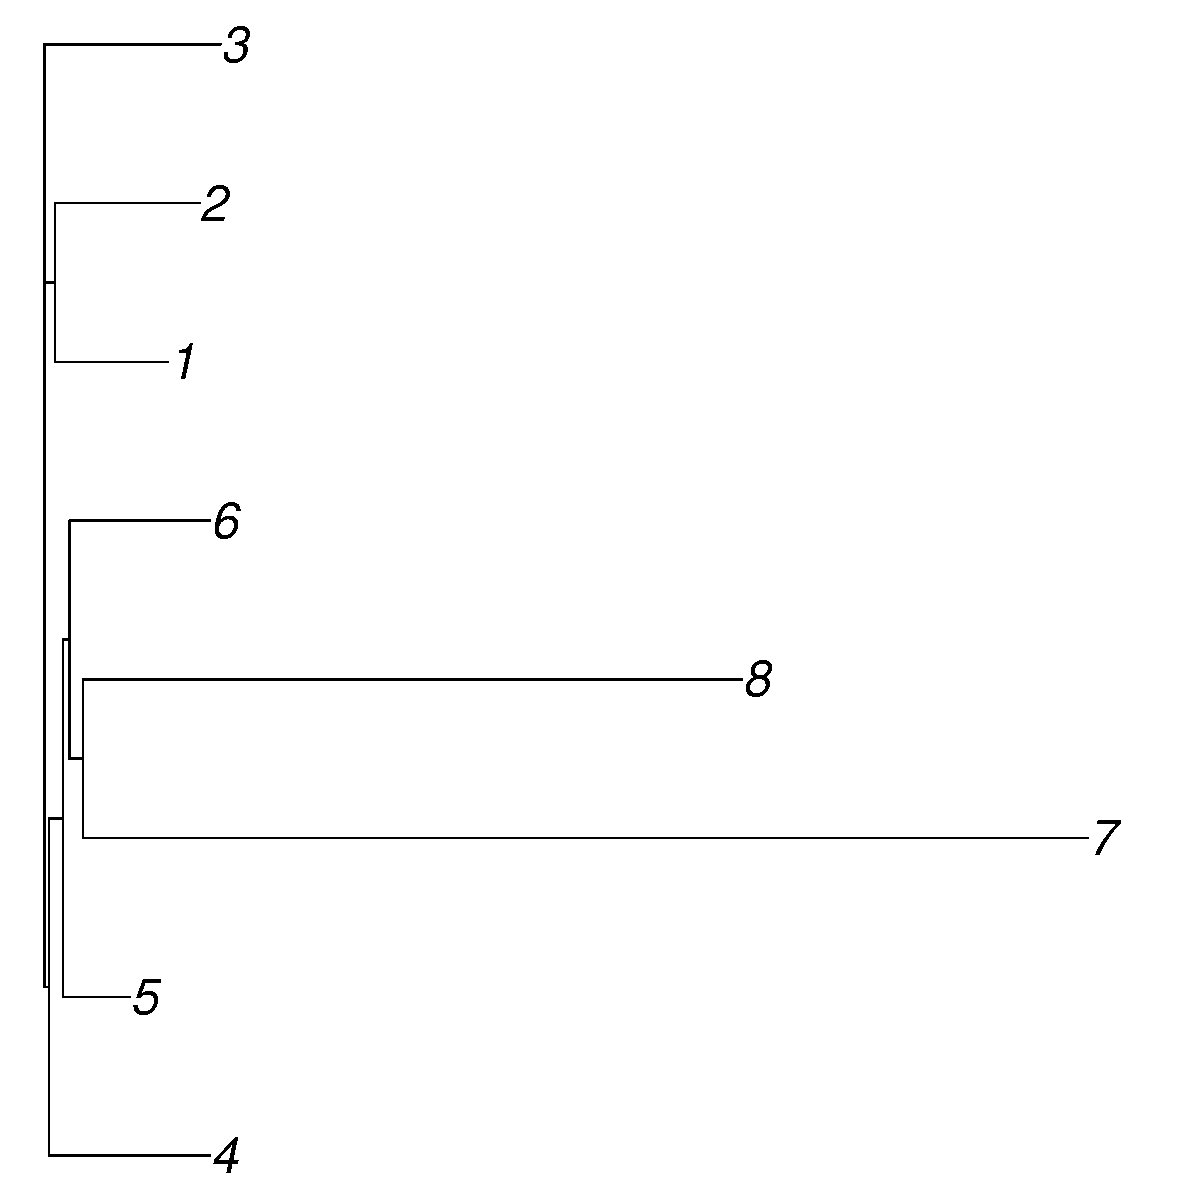
\includegraphics[width=\linewidth]{../../../talks/eucalyptus/colloquium_2016/figures/gatk_tree2.pdf}
% % 	\column{.5\linewidth}
% % 		\includegraphics[width=\linewidth]{../../../talks/eucalyptus/colloquium_2016/figures/labeled_tree.jpg}
% % 	\end{columns}
% % \end{frame}

% % \begin{frame}{Branch 7}
% % Branch 7 is consistently in the wrong place. Why? What's going on with that branch?
% % \begin{definition}
% % 	\textbf{Long Branch Attraction} is the tendency of long branches to cluster in a phylogenetic tree
% % \end{definition}

% % \begin{itemize}
% % \item Branch 7 is the longest branch
% % \item May be affected by assumptions about zygosity
% % \item Do particular genomic regions make mutation calling more difficult for one method?
% % \end{itemize}
% % \end{frame}

% \begin{frame}{If you want something done right...}

% Use \textit{E. melliodora} genome as a starting place, then generate a new reference and map to that reference.

% \begin{tikzpicture}[cnode/.style={rectangle,draw=black!60,fill=black!5,very thick}, node distance = .5 cm]
% 	\node[cnode] (reads){Reads};
% 	\node[cnode] (eg)[below = of reads]{E. grandis};
% 	\node[cnode] (em1)[right = of eg]{E. melliodora 1};
% 	\node[cnode] (em2)[right = of em1]{E. melliodora 2};
% 	\node[cnode] (etc)[right = of em2] {...};
% 	\draw[very thick,->] (reads) to [out=180,in=190] (eg);
% 	\draw[very thick,->] (reads) to [out=180,in=170] (eg);
% 	\draw[very thick,->] (reads) to [in=80] (em1);
% 	\draw[very thick,->] (reads) to [in=110] (em1);
% 	\draw[very thick,->] (eg) -- (em1);
% 	\draw[very thick,->] (em1) -- (em2);
% 	\draw[very thick,->] (em2) -- (etc);
% \end{tikzpicture}

% % \begin{alertblock}{Next Steps}
% % \begin{itemize}
% % \item Generate a genome and recursively improve it with multiple tools
% % \item Filter repetitive elements that complicate mapping
% % \item How do the mutations found with DiscoSNP compare to those found with GATK? Is there a pattern?
% % \item Validation
% % \end{itemize}
% % \end{alertblock}

% \end{frame}

% \begin{frame}{Our New Reference Improves Mapping Quality}
% \begin{center}
% \includegraphics[height=.9\textheight]{../../../talks/eucalyptus/colloquium_2016/figures/both_hist.pdf}
% \end{center}
% \end{frame}

% \begin{frame}{Next Steps}
% \begin{itemize}
% \item Continue improving the reference we've created.
% \item Filter out repetitive elements that make mapping difficult
% \item Once we are confident in our data, make a prediction about the herbivore resistance
% \item Validate
% \end{itemize}
% \end{frame}

% \begin{frame}{Conclusions}
% \begin{itemize}
% \item A reference-free method performs similarly to a standard pipeline
% \item Aligning to a reference, then using that alignment as a reference for another alignment can improve mapping qualities.
% \end{itemize}
% \end{frame}

% % \begin{frame}{Acknowledgements}
% % \begin{itemize}
% % \item Reed Cartwright
% % \item Human and Comparative Genomics Laboratory
% % \item Robert Lanfear, Macquarie University
% % \end{itemize}

% % \begin{columns}
% % \column{.4\linewidth}
% % 	
\includegraphics[width=.9\linewidth]{../../../talks/eucalyptus/colloquium_2016/figures/lab_logo.pdf}
% % 	
\includegraphics[width=.9\linewidth]{../../../talks/eucalyptus/colloquium_2016/figures/biodesign_logo.pdf}
% % \column{.4\linewidth}
% % 	
\includegraphics[width=.9\linewidth]{../../../talks/eucalyptus/colloquium_2016/figures/sols_logo.pdf}
% % \end{columns}

% % \end{frame}

% %Graph Theory
% %How does a reference free method work?
% %The tree I got
% %Compare to GATK
% %Why is this happening? IDK
% %Talk about improving the assembly

\end{document}